\documentclass{beamer}
\usetheme{Darmstadt}
\usecolortheme{default}
\usepackage{draftcopy}
\usepackage{graphicx}
\usepackage{amsmath}
\usepackage{enumerate}
\usepackage{verbatim}
\beamertemplatenavigationsymbolsempty


%This script was pulled from pdflatex codes

%\MyLogo{ECO364 (International Trade) Summer 2016}
%\leftheader{Using CVS in Autominder}
%\rightheader{Using CVS in Autominder\quad\textsf{\tiny[\thepage]}}
%\rightheader{\quad\textsf{\tiny[\thepage]}}
%\rightfooter{\quad\textsf{\thepage}}

% Set the default page color and style.
%\pagecolor{white}
%\vpagecolor[lightblue]{green}
%\vpagecolor{bgblue}
%
%\hpagecolor[cyan]{white}


\title{ECO364 (International Trade) Summer 2016}
\date{June 9, 2016}
\author[Scott Orr]{Scott Orr}
\institute{University of Toronto}

\AtBeginSection[]
{
	\begin{frame}
		\frametitle{Outline}
		\tableofcontents[currentsection]
	\end{frame}
}

\begin{document}
	
	\begin{frame}
		\titlepage
	\end{frame}
	
\section{Outline}

\begin{frame}
\frametitle{Outline for Today}
\begin{itemize}
	\item Finish monopolistic competition model with homogeneous firms
		\begin{itemize}
			\item Implications of the model with trade.
				\begin{itemize}
					\item ``Pro-competitive" gains from trade.
					\item Gains from variety.
					\item Efficiency gains. 
				\end{itemize}
		\end{itemize}
	\item Monopolistic competition with heterogeneous firms
		\begin{itemize}
			\item New result: Allocative gains from trade.	
				\begin{itemize}
					\item Trade integration tends to force less productive firms out the market. 
				\end{itemize}
		\end{itemize}
\end{itemize}
\end{frame}



\section{Monopolistic Competition with Homogeneous Firms}
\subsection{Set up}

\begin{frame}
\frametitle{Review of last class}

Last class we walked through the solving the monopolistic competition model.
\begin{itemize}
	\item Model has three ``key" unknowns: $(n,p,AC)$
	\item Pin down the endogenous variables with three equations:
		\begin{itemize}
			\item The ``average cost curve": $AC=c+n\frac{F}{S}$
			\item The ``price curve" $p=c+\frac{1}{bn}$:
			\item Free entry and exit (zero profit condition): $p=AC$
		\end{itemize}
\end{itemize}
Intersection of average cost curve and price curve determines equilibrium $n^*$

\end{frame}

\begin{frame}
	\frametitle{Equilibrium}
	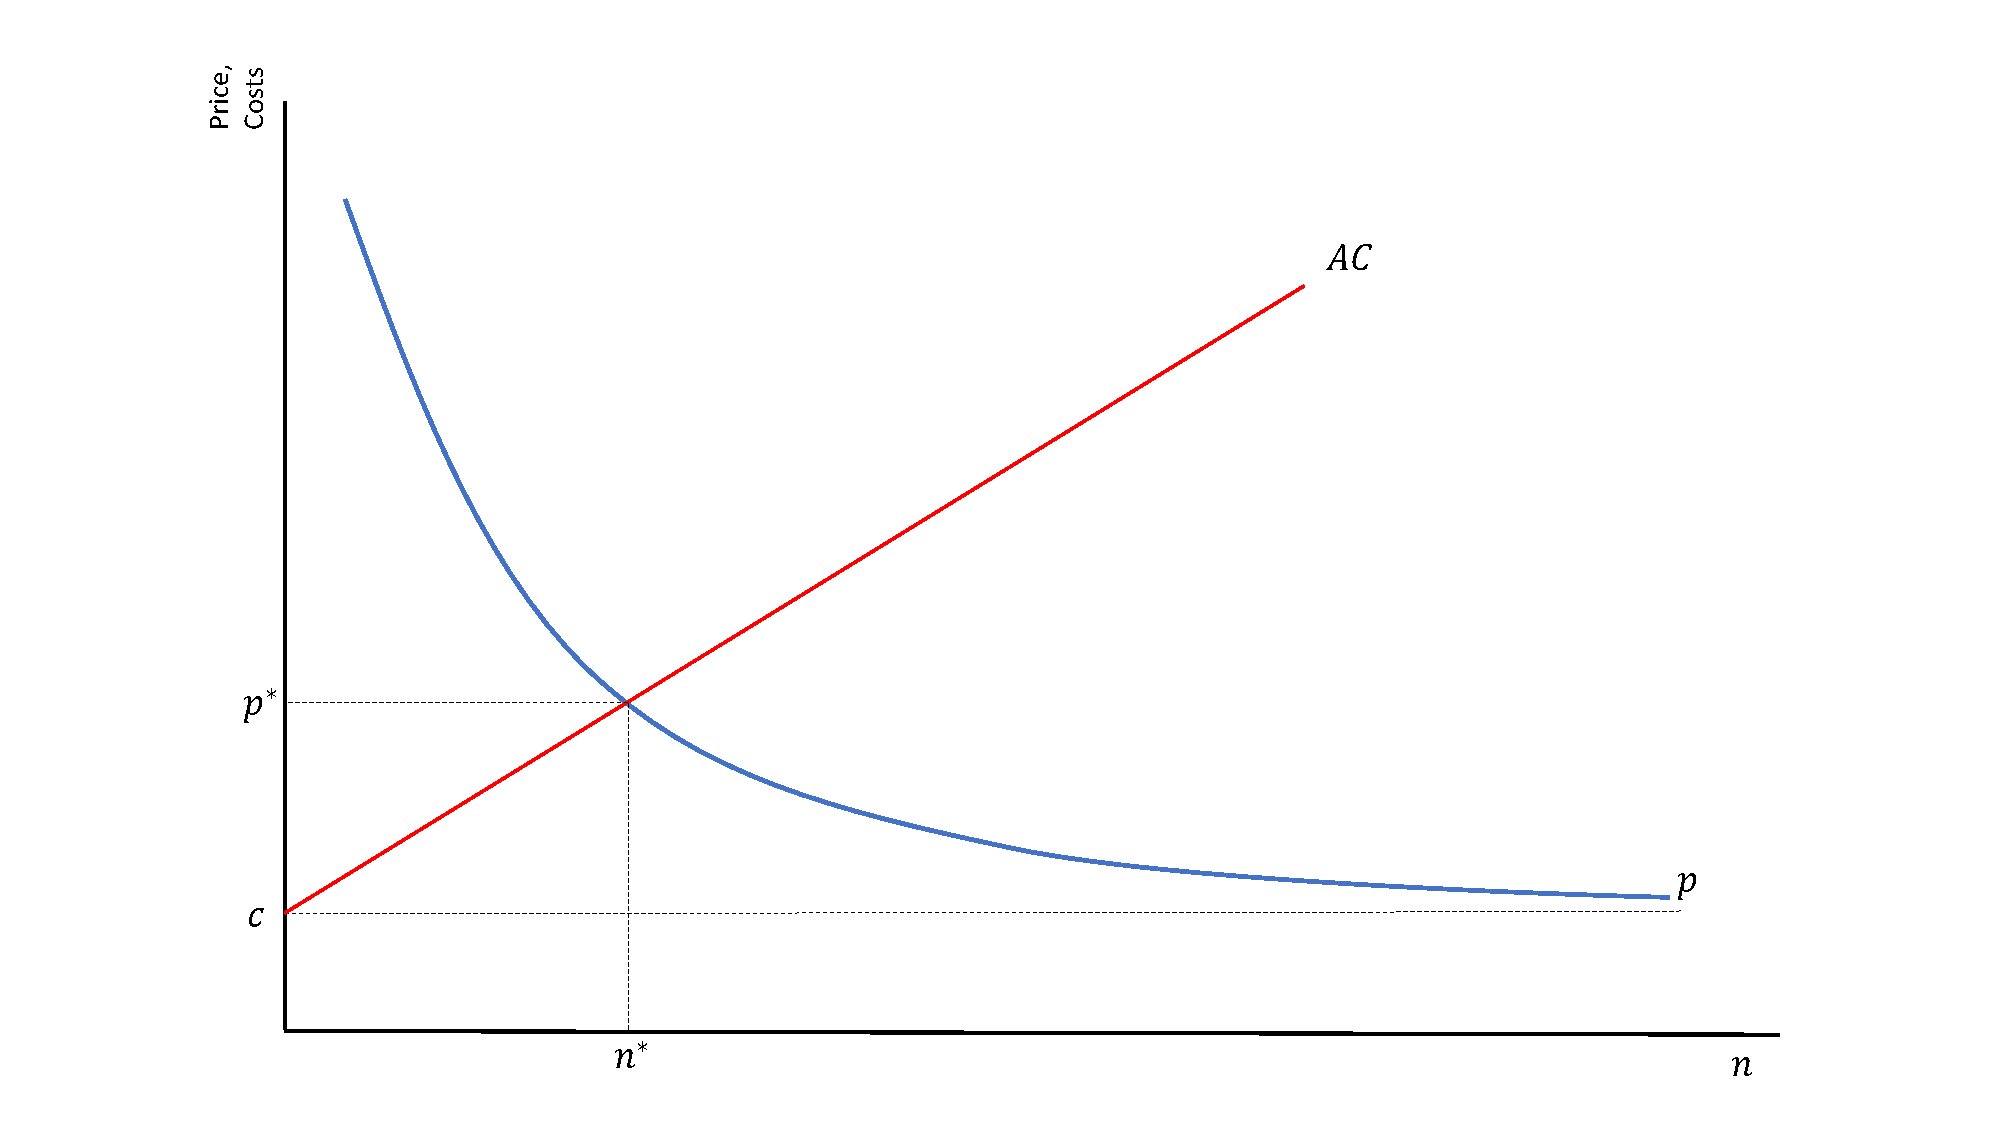
\includegraphics[scale=0.3]{SL2_7.pdf}
	
	\scriptsize
	Or analytically:
	\begin{equation}
	n^* =\left(\frac{S}{Fb}\right)^{1/2}, \nonumber \qquad
	p^*=c + \left(\frac{F}{bS}\right)^{1/2}
	\end{equation}
	
	
\end{frame}
\subsection{Monopolistic Competition and Trade}
\begin{frame}
	\frametitle{Monopolistic Competition and Trade}
	Trade can be seen as an increase in market size (Krugman 1979)
	\begin{itemize}
		\item Suppose $S_1$ people live in country 1 and $S_2$ live in country 2.
			\begin{itemize}
				\item Total market size for free trade equilibrium = $S_1 + S_2$
				\item Essentially the same equilibrium except $S\uparrow$
			\end{itemize}
		\item Recall:
		$$AC=c+n\frac{F}{S}$$
		$$p=c+\frac{1}{bn}$$
		\item Average cost curve \emph{rotates} downwards, price curve remains constant
	\end{itemize}
	
\end{frame}

\begin{frame}
	\frametitle{Monopolistic Competition and Trade}
	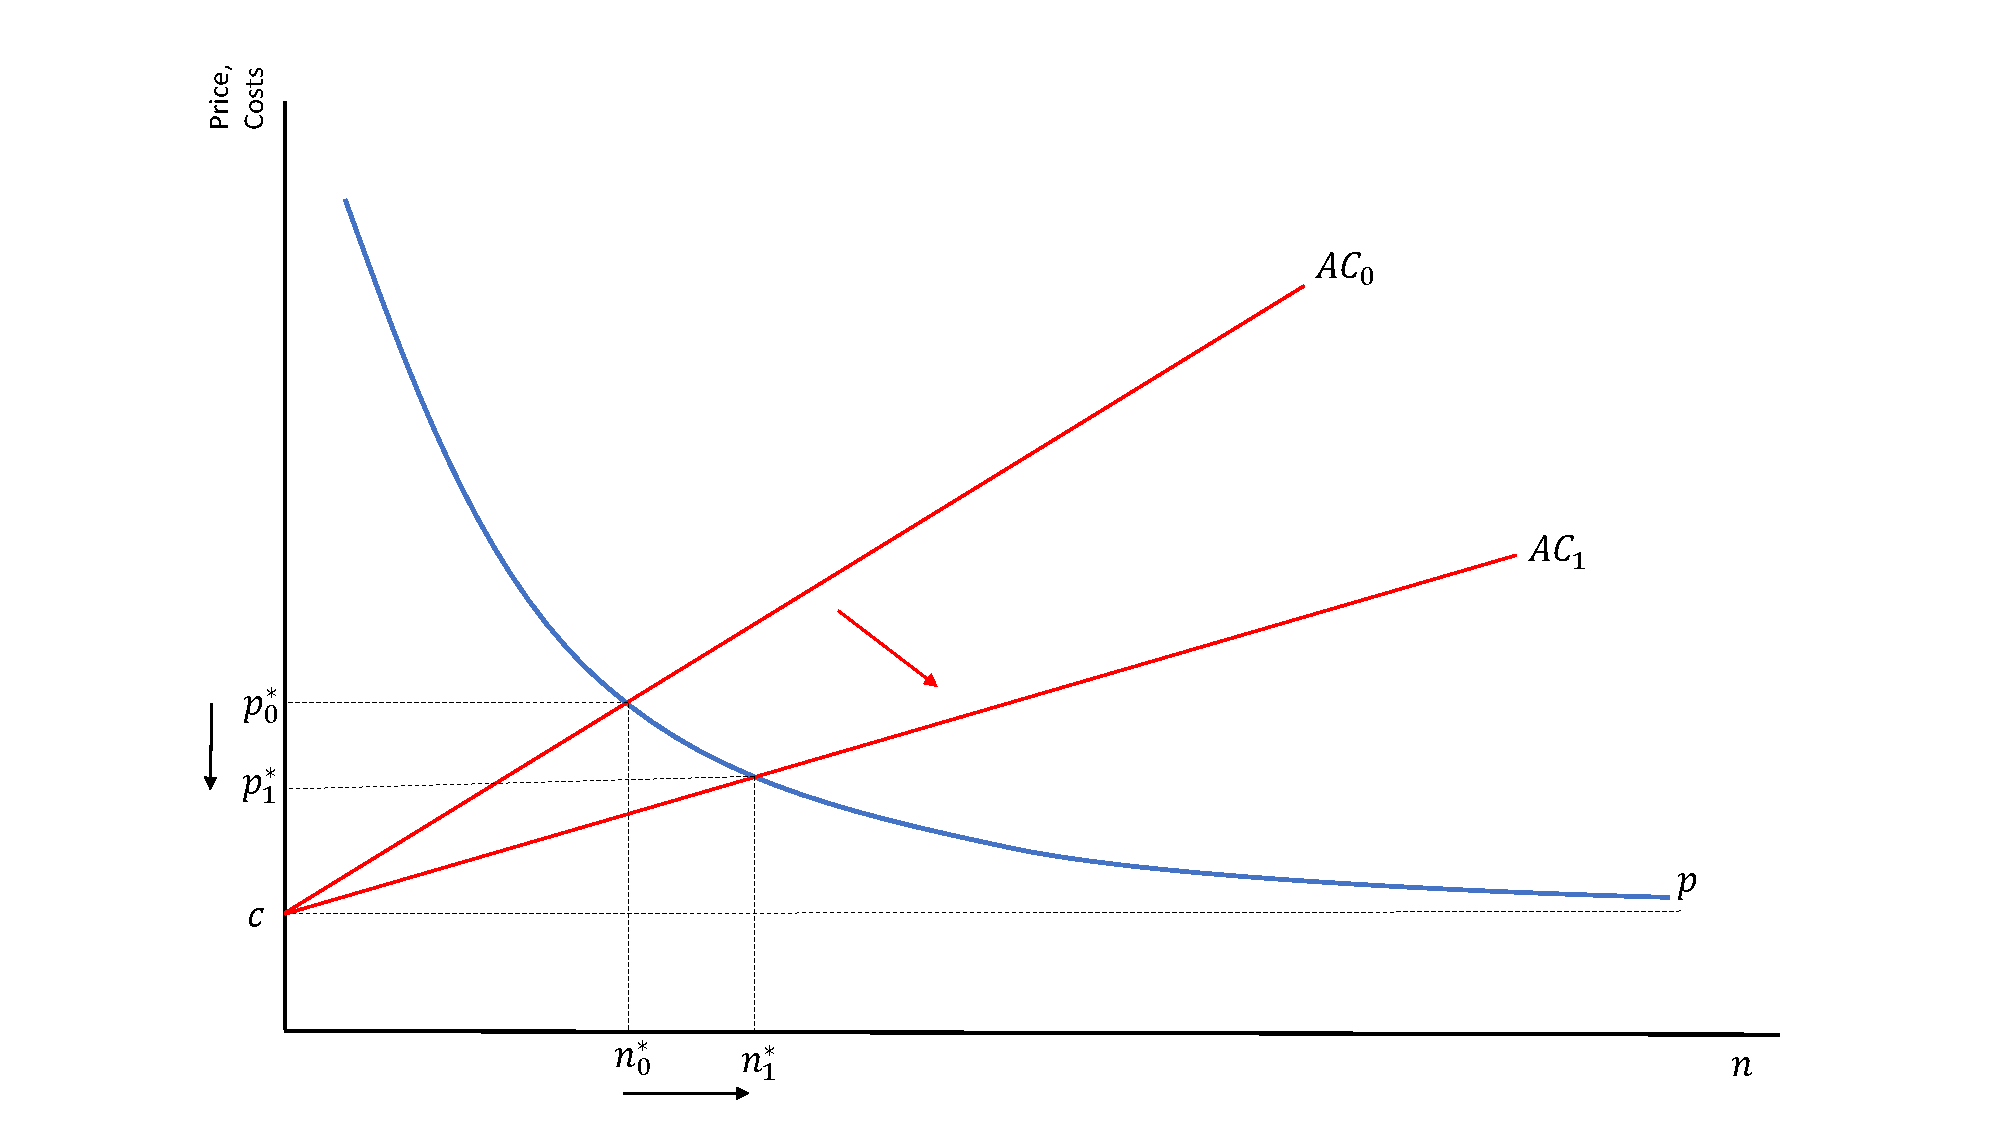
\includegraphics[scale=0.32]{SL2_8.pdf}
\end{frame}


\begin{frame}
	\frametitle{Gains from trade with monopolistic competition}
	\begin{itemize}
		\item When two countries open up to trade, consumers now get to purchase more varieties than in the autarky equilibrium.
		\begin{itemize}
			\item $\uparrow n$: Consumers gain from more varieties/firms.
		\end{itemize}
		\item Because under free trade each firm produces at a larger scale, it can exploit economies of scale further, cutting costs.
		\begin{itemize}
			\item Recall $q=\frac{S}{n}$
			\begin{itemize}
				\item While both $S$ and $n$ rise, can show that $\uparrow S > \uparrow n$ (Problem Set 4)
			\end{itemize}
		\end{itemize}
		
		\item Consumer gain from lower prices.
		\begin{itemize}
			\item Recall that markups are given by: $\mu=\frac{1}{bn}$
			\item $\uparrow n$, increased competition, firms decrease their markups, and prices fall.
			\item So called ``Pro-competitive" gains from trade. 
		\end{itemize}
	\end{itemize}
	
\end{frame}

\begin{frame}
	\frametitle{Market size, trade integration, and competition}
	We have just considered opening up to trade as an increase in market size, and showed that this increases the number of firms selling to a \emph{particular country} in equilibrium.
	\begin{itemize}
		\item Note that there will generally be more firms operating \emph{across} the two countries before integration.
		\begin{itemize}
			\item While varieties available to each consumer increases, increased competition causes some firms to exit the market.
			\item We tend to see effects of this sort in practice:
			\begin{itemize}
				\item Following NAFTA, General Motors cut in half the number of car models produced in Canada. 
			\end{itemize}
		\end{itemize}
	\end{itemize}
\end{frame}

\begin{frame}
	\frametitle{Exit-Effects Following Trade LIberalization}	
	
	Consider two completely identical countries:
	\begin{itemize}
		\item Autarky number of firms in each country:
		\begin{itemize}
			\item $n^A=\left(\frac{S}{Fb}\right)^{1/2}$
			\item Overall number of firms $2n^A=2n^A=2\left(\frac{S}{Fb}\right)^{1/2}$
		\end{itemize}
		\item Total number of firms in the free-trade \emph{integrated} equilibrium
		\begin{itemize}
			\item $n^T=\left(\frac{2S}{Fb}\right)^{1/2}$
		\end{itemize}
		\item Note that since $\sqrt{2}<2$
		\scriptsize
		\begin{equation}
		n^T = \left(\frac{2S}{Fb}\right)^{1/2} = \sqrt{2}\left(\frac{S}{Fb}\right)^{1/2} < 2\left(\frac{S}{Fb}\right)^{1/2}  = 2n^A \nonumber
		\end{equation}
		\normalsize
		\item Clearly some firms will have to exit the market following trade-liberalization!
		\begin{itemize}
			\item However, since $n^A<n^T$, there are still variety gains from trade, \emph{even though countries are identical}
		\end{itemize}
	\end{itemize}
	
\end{frame}

\begin{frame}
	\frametitle{Example: Gains from variety vs. world loses in variety}
	\footnotesize
\begin{itemize}
	\footnotesize
	\item In Autarky:
		\begin{itemize}
			\footnotesize
			\item U.S. produces: 
				\begin{itemize}
					\footnotesize
					\item Ford Pintos
					\item Chevrolet Suburbans
				\end{itemize}
				
			\item Germany produces:
				\begin{itemize}
					\footnotesize
					\item Volkswagen Rabbits
					\item BMWs
				\end{itemize}
		\end{itemize}
	\item With Trade:
			\begin{itemize}
				\footnotesize
				\item U.S. produces: 
				\begin{itemize}
					\footnotesize
					\item Chevrolet Suburbans
				\end{itemize}
				\item Germany produces:
				\begin{itemize}
					\footnotesize
					\item Volkswagen Rabbits
					\item BMWs
				\end{itemize}
			\end{itemize}

Both the U.S. and Germany enjoy gains from variety ($2 \rightarrow 3 $ car varieties), even though world variety falls ($4\rightarrow 3$).
		

\end{itemize}
\end{frame}



\begin{frame}
	\frametitle{Exit-Effects Following Trade Liberalization}
	While some firms will exit the market following trade integration, model makes no predictions as to \emph{who} will exit the market.
	\begin{itemize}
		\item Empirical literature has generally found that \emph{less productive} firms are most likely to exit the market following trade liberalization (E.g. Pavcnik 2002).
		\item To make sense of these facts, we need a model that accounts for \emph{firm heterogeneity}
	\end{itemize}
\end{frame}

\section{Monopolistic Competition With Firm Heterogeneity}
\subsection{Set up}
\begin{frame}
	\frametitle{Monopolistic Competition with Heterogeneous Firms: Set-up}
	
The demand system for firm $j$ is the heterogeneous firm model is identical to the homogeneous firm model:

\begin{equation}
q_j(p_j)=S\left[\frac{1}{n} - b\left(p_j -\bar{p} \right)\right] \nonumber
\end{equation}

The only difference is the total cost function, which now differs from firm-to-firm

\begin{itemize}
	\item To simplify for now, assume that there are no fixed costs of production (constant returns to scale)
	\begin{equation}
	TC_j=c_jq_j		\nonumber
	\end{equation}
\end{itemize}

\emph{Marginal costs} differ across firms
		
\end{frame}

\begin{frame}
	\frametitle{Firm-level pricing}
Since different firms have different costs, cannot assume symmetric pricing.
\begin{itemize}
	\item Each firm still prices according to the first-order condition:
		\begin{itemize}
			\item $MR_j=MC_j$
		\end{itemize}
	\item Given the demand function described in the last slide, this becomes:
	\begin{equation}
	p_{j}-\frac{q_{j}}{bS}=c_j \nonumber
	\end{equation}
	\item This first order condition written in this way is not very informative, since both $q_j$ and $p_j$ are endogenous.
		\begin{itemize}
			\item Substitute in $q_j(p_j)$ and solve for $p_j$
		\end{itemize}
		
		\begin{equation}
		p_j^*=p^*(c_j)=\frac{1}{2}\left(\frac{1}{bn}+\bar{p} + c_j\right) \nonumber 
		\end{equation}
	\item Firms with higher costs charge higher prices!
\end{itemize}
\end{frame}

\begin{frame}
	\frametitle{Pricing, Quantity, and Profits by Costs}
	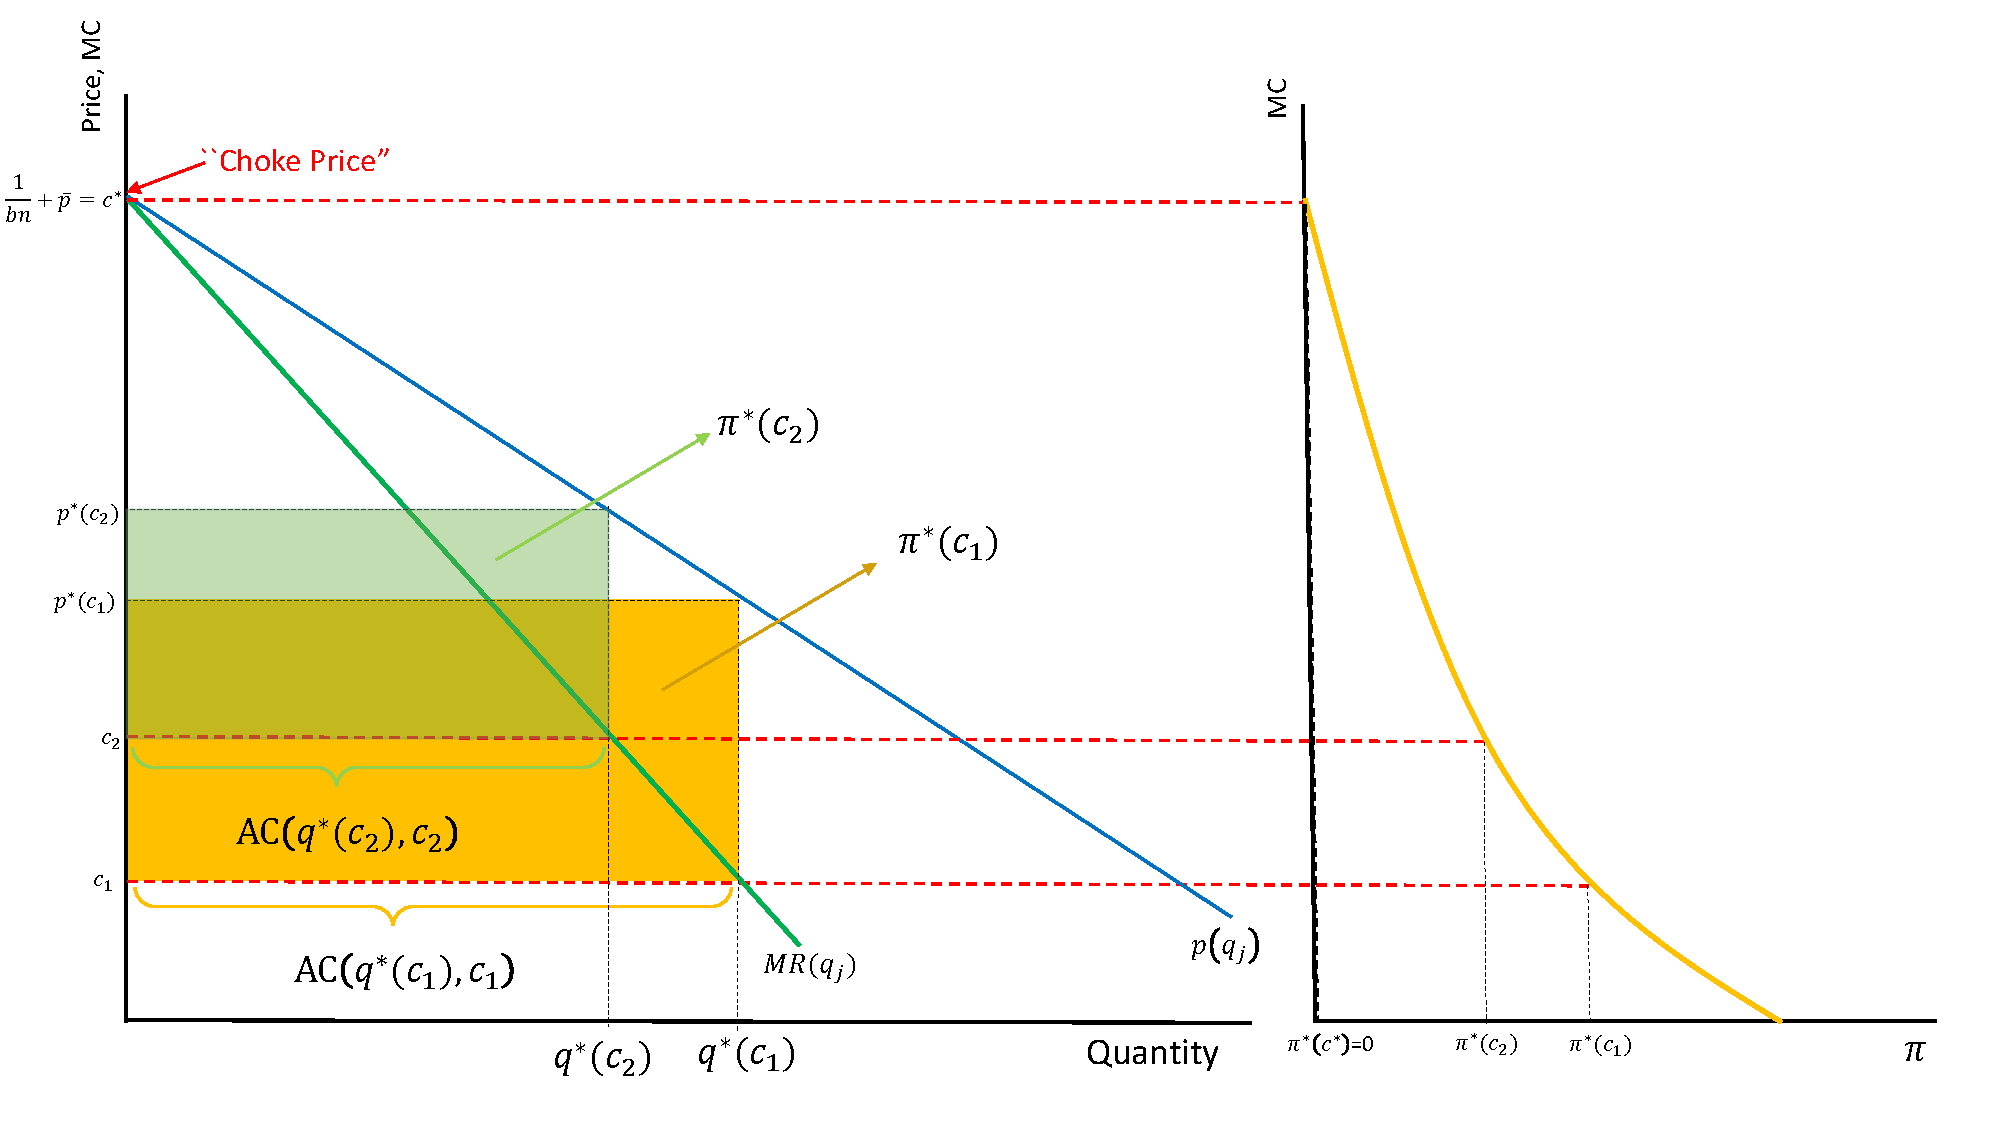
\includegraphics[scale=0.32]{SL3_1.pdf}

\end{frame}

\begin{frame}
	\frametitle{Choke Prices, Profits and Marginal Cost}
\begin{itemize}
	\item Note that if a producer charges any price above the inverse demand intercept ($\frac{1}{bn}+\bar{p}$), \emph{no consumers will buy the product}. 
		\begin{itemize}
			\item This price is called the ``choke price"
			\item Due to choke price, impossible for producers with $c>\frac{1}{bn}+\bar{p}$ to make profits.
				\begin{itemize}
					\item These sellers will exit the market.
				\end{itemize}
		\end{itemize}
	\item In general, profits will be decreasing in marginal costs. 
		\begin{itemize}
			\item $\pi(c_j)=(p^*(c_j)-c_j)q^*(c_j)$
			\item Using the fact that $p^*(c_j)=\frac{1}{2}\left(\frac{1}{bn}+\bar{p} + c_j\right)$, easy to show:
		\end{itemize}
\end{itemize}
			\begin{equation}
			\pi(c_j)=\frac{Sb}{4}\left(\frac{1}{bn}+\bar{p} -c_j \right)^2 \nonumber
			\end{equation}
			\begin{itemize}
				\item Notice that profits are increasing with market size, but fall as competition rises ($\uparrow n$ and $\downarrow \bar{p}$)
			\end{itemize}
			
\end{frame}
\subsection{Monopolistic Competition and Trade}
\begin{frame}
	\frametitle{Impact of Trade: Larger market with more competition}
To gain some intuition,  let's think of trade integration as an increase in market size $S$ as well as an increase in $n$ (similar to homogeneous firm model)
	\begin{itemize}
				\item Think of this as a ``really" short-run model, where firms are not allowed to exit yet, so $n$ has to increase because home consumers can buy foreign varieties of a product as well. 
				\item We shall show in a moment that trade integration ($\uparrow S$) will actually imply that $\frac{1}{bn}+\bar{p}$ has to fall.
					\begin{itemize}
						\item Requires that we pin down the endogenous variables $\{n,\bar{p}\}$ using an \emph{expected} zero profit condition.
						\item A bit complicated to show this result formally, so let's first focus understanding the \emph{intuition} for what trade integration does to the Home economy.  
					\end{itemize}
	\end{itemize}


\end{frame}

\begin{frame}
	\frametitle{The impact of trade on heterogeneous firms}
 Broadly speaking, there are two opposing forces at work here:
		\begin{enumerate}
			\item $\uparrow S$: Now firms can sell to more people, $\uparrow \pi$
			\item $\uparrow n $ competition: More firms charging lower prices,  $\downarrow \pi$
		\end{enumerate}
The interaction between these forces creates \emph{winners and losers} due to trade integration. 
	\begin{itemize}
		\item Really productive firms (low $c$) benefit more from increased market size than low productivity firms (high $c$)
	\end{itemize}

\end{frame}

\begin{frame}
	\frametitle{Larger Market and More Competition: Winners and Losers}
	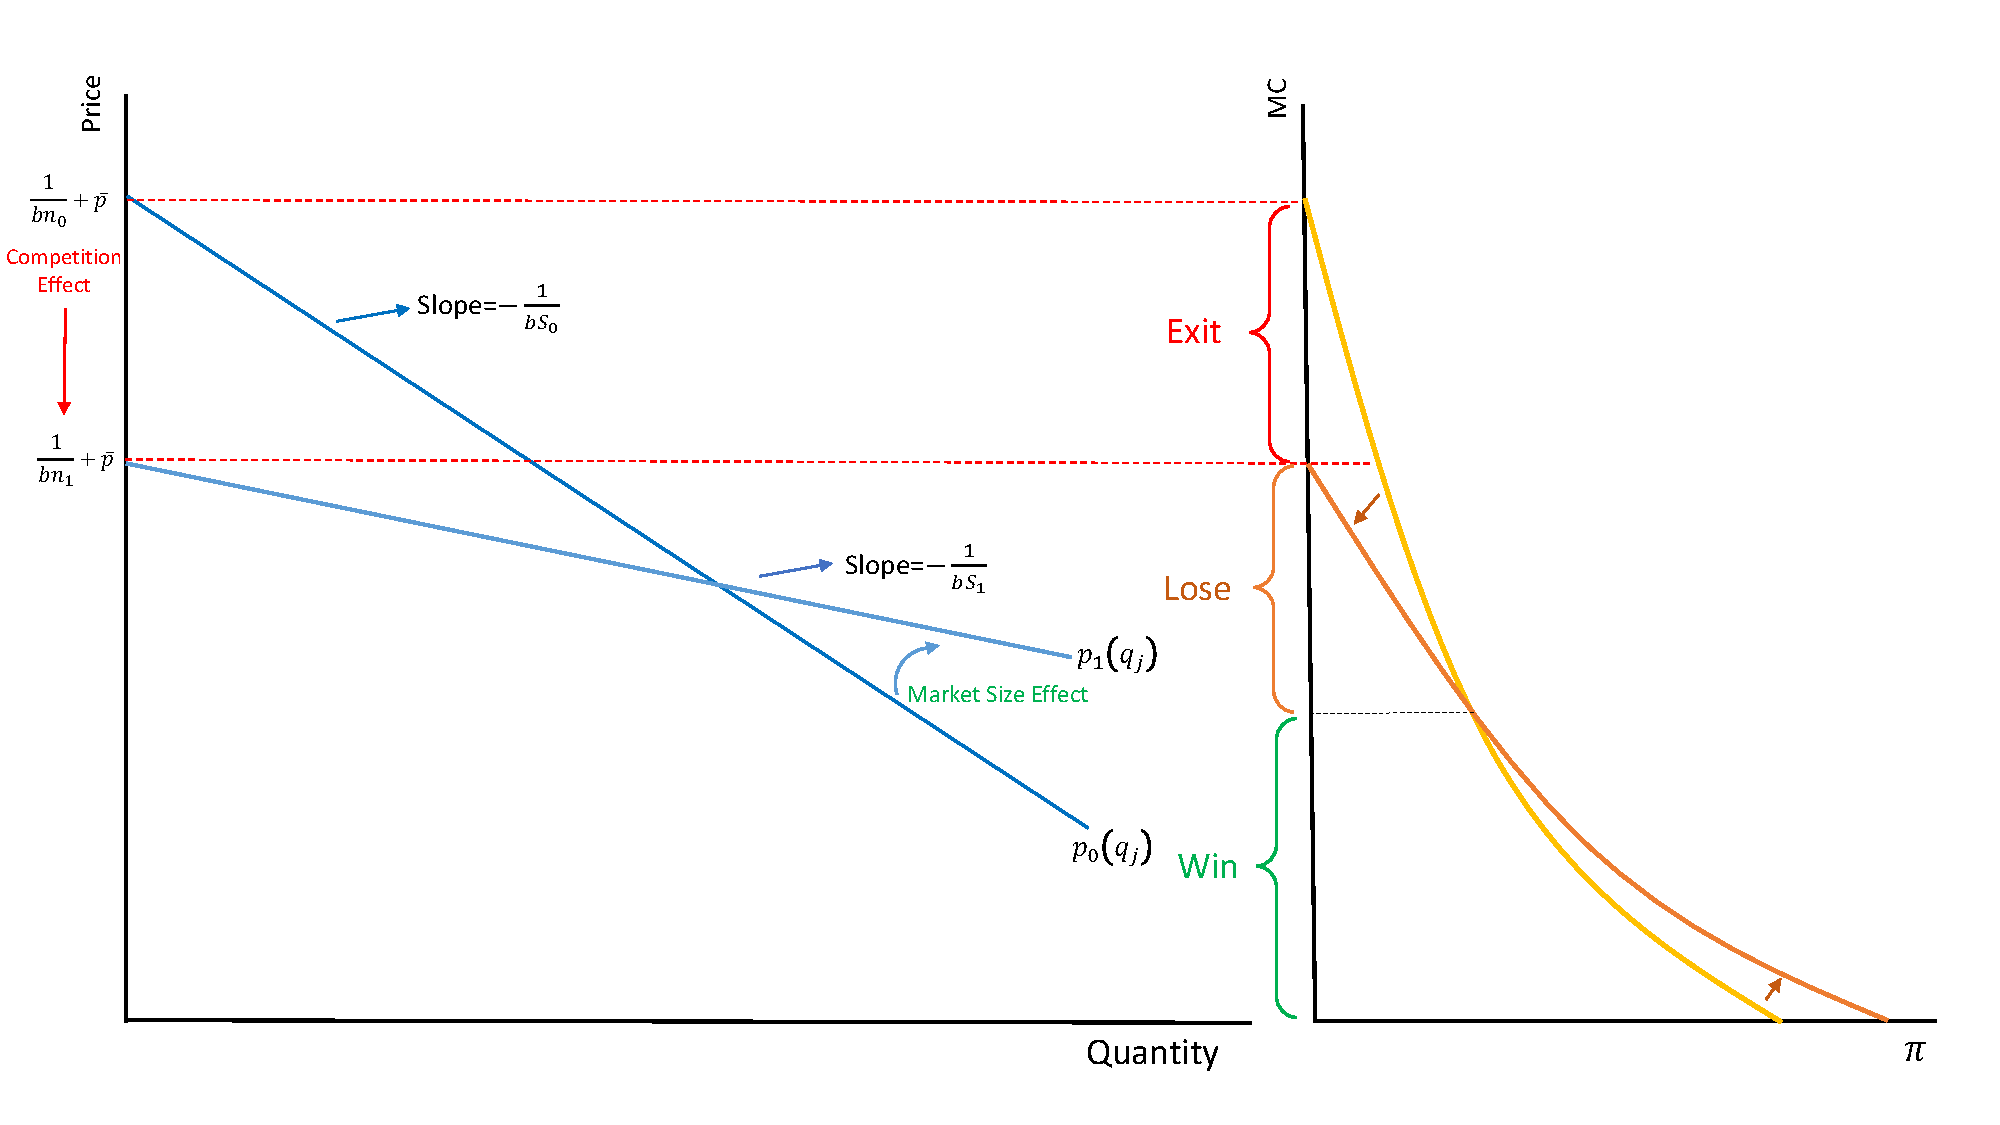
\includegraphics[scale=0.32]{SL3_2.pdf}
\end{frame}

\begin{frame}
	\frametitle{Winners and Losers with Trade: Intuition}
\begin{itemize}
	\item Net effect of increased competition and increased market size \emph{rotates} demand.
		\begin{itemize}
			\item Roughly, firms selling small quantities primarily experience a demand \emph{contraction}
			\item Firms selling large quantities (the efficient firms) experience a demand \emph{expansion}
		\end{itemize}
	\item Inefficient firms are forced out of the market, but efficient firms gain more market share
		\begin{itemize}
			\item Trade can increase average productivity!
				\begin{itemize}
					\item More formal demonstrations of these ideas (in general equilibrium) can be found in Melitz (2003) and Melitz and Ottaviano (2008)
				\end{itemize}
		\end{itemize}
\end{itemize}
\end{frame}

\begin{frame}
	\frametitle{Does trade increase comeptition in the heterogeneous firm model?}
If trade integration is simply an increase in $S$, does competition have to increase?
	\begin{itemize}
		\item In the homogeneous firm model, we showed that $\uparrow S$ implies that $\uparrow n$ and $\downarrow \bar{p}$.
			\begin{itemize}
				\item Somewhat difficult to show what happens to these variables separately, but we can show what happens to ``competition", or $\frac{1}{bn} +\bar{p}$
				\item However, to do this, we need an extra condition to pin down these endogenous variables.
			\end{itemize}
			\item With homogeneous firms, we invoked symmetry and free-entry.
					\begin{itemize}
						\item Not possible to invoke symmetry now, since firms clearly behave differently!
					\end{itemize}
					\item We need a new type of free-entry condition to solve the model. 
	\end{itemize}
	
\end{frame}

\begin{frame}
	\frametitle{Closing the heterogeneous firm model: Free-Entry}
	Solution: Model entry as a two-stage process, and set \emph{expected} profits equal to zero.
	\begin{itemize}
		\item Stage 1:
		\begin{itemize}
			\footnotesize
			\item All (potential) firms are identical \emph{ex-ante} 
			\item Potential firms decide whether they want to enter the market or not.
			\item If they choose to enter they must pay a \emph{sunk} entry cost $K$  on research and development. Otherwise they get a payoff of zero. 
			\item After paying the entry cost, each firm makes a \emph{marginal cost draw} from the same known distribution (e.g. a normal distribution)
		\end{itemize}
		\item Stage 2:
		\begin{itemize}
			\footnotesize
			\item All cost draws are realized.
			\item Firms who draw  $c_j >\frac{1}{bn}+\bar{p}$ exit.
			\item $c_j \leq\frac{1}{bn}+\bar{p}$
		\end{itemize}
	\end{itemize}
\end{frame}

\begin{frame}
	\frametitle{Expected Free Entry Equilibrium}
We assume that firms enter the market until \emph{expected} profits are zero.
	\begin{itemize}
		\item While all the firms who \emph{remain} in the market in stage 2 earn positive profits, some firms will earn negative profits \emph{from the perspective of stage 1} !
			\begin{itemize}
				\item Firms who draw $c>\frac{1}{bn}+\bar{p}$ and exit earn $-K$.
			\end{itemize}
		\item Since some firms ``win" and some firms "lose" we are looking for the value of ``competition" that makes the expected benefit of this gamble exactly equal to zero.
			\begin{itemize}
				\item Expected stage 2 profits (operating profits) must equal $K$
			\end{itemize}
		\end{itemize}
\end{frame}

\begin{frame}[label=cost]
	\frametitle{Cost Cutoffs and Expected Profits}
Define the ``cut-off" marginal cost, $c^*$ as the marginal cost draw where a firm is just indifferent between staying and exiting the market. 
\begin{itemize} 
	\item We know from our earlier calculations that is must be that  $c^*=\frac{1}{bn}+\bar{p}$ (Recall the ``choke price")
		\begin{itemize}
			\item If we can solve for the cut-off marginal cost, we will now know level of competition prevails in the market (i.e. we know the intercept of the demand curve).
		\end{itemize}
	\item It is straightforward to show that expected profits are \emph{increasing} in the cut-off marginal cost. \hyperlink{Formal}{\beamerbutton{Formal Demonstration}}
		\begin{itemize}
			\item For any active firm, operating profits increase with $c^*$ since $\pi(c_j)=\frac{Sb}{4}\left(\frac{1}{bn}+\bar{p} -c_j \right)^2 =  \frac{Sb}{4}\left(c^*-c_j \right)^2 $
			\item Increasing $c^*$ turns ``exiters" into "stayers", which strictly increases their profit as well.
		\end{itemize}


\end{itemize}

\end{frame}

\begin{frame}
	\frametitle{Expected profits rise as less productive firms survive}
		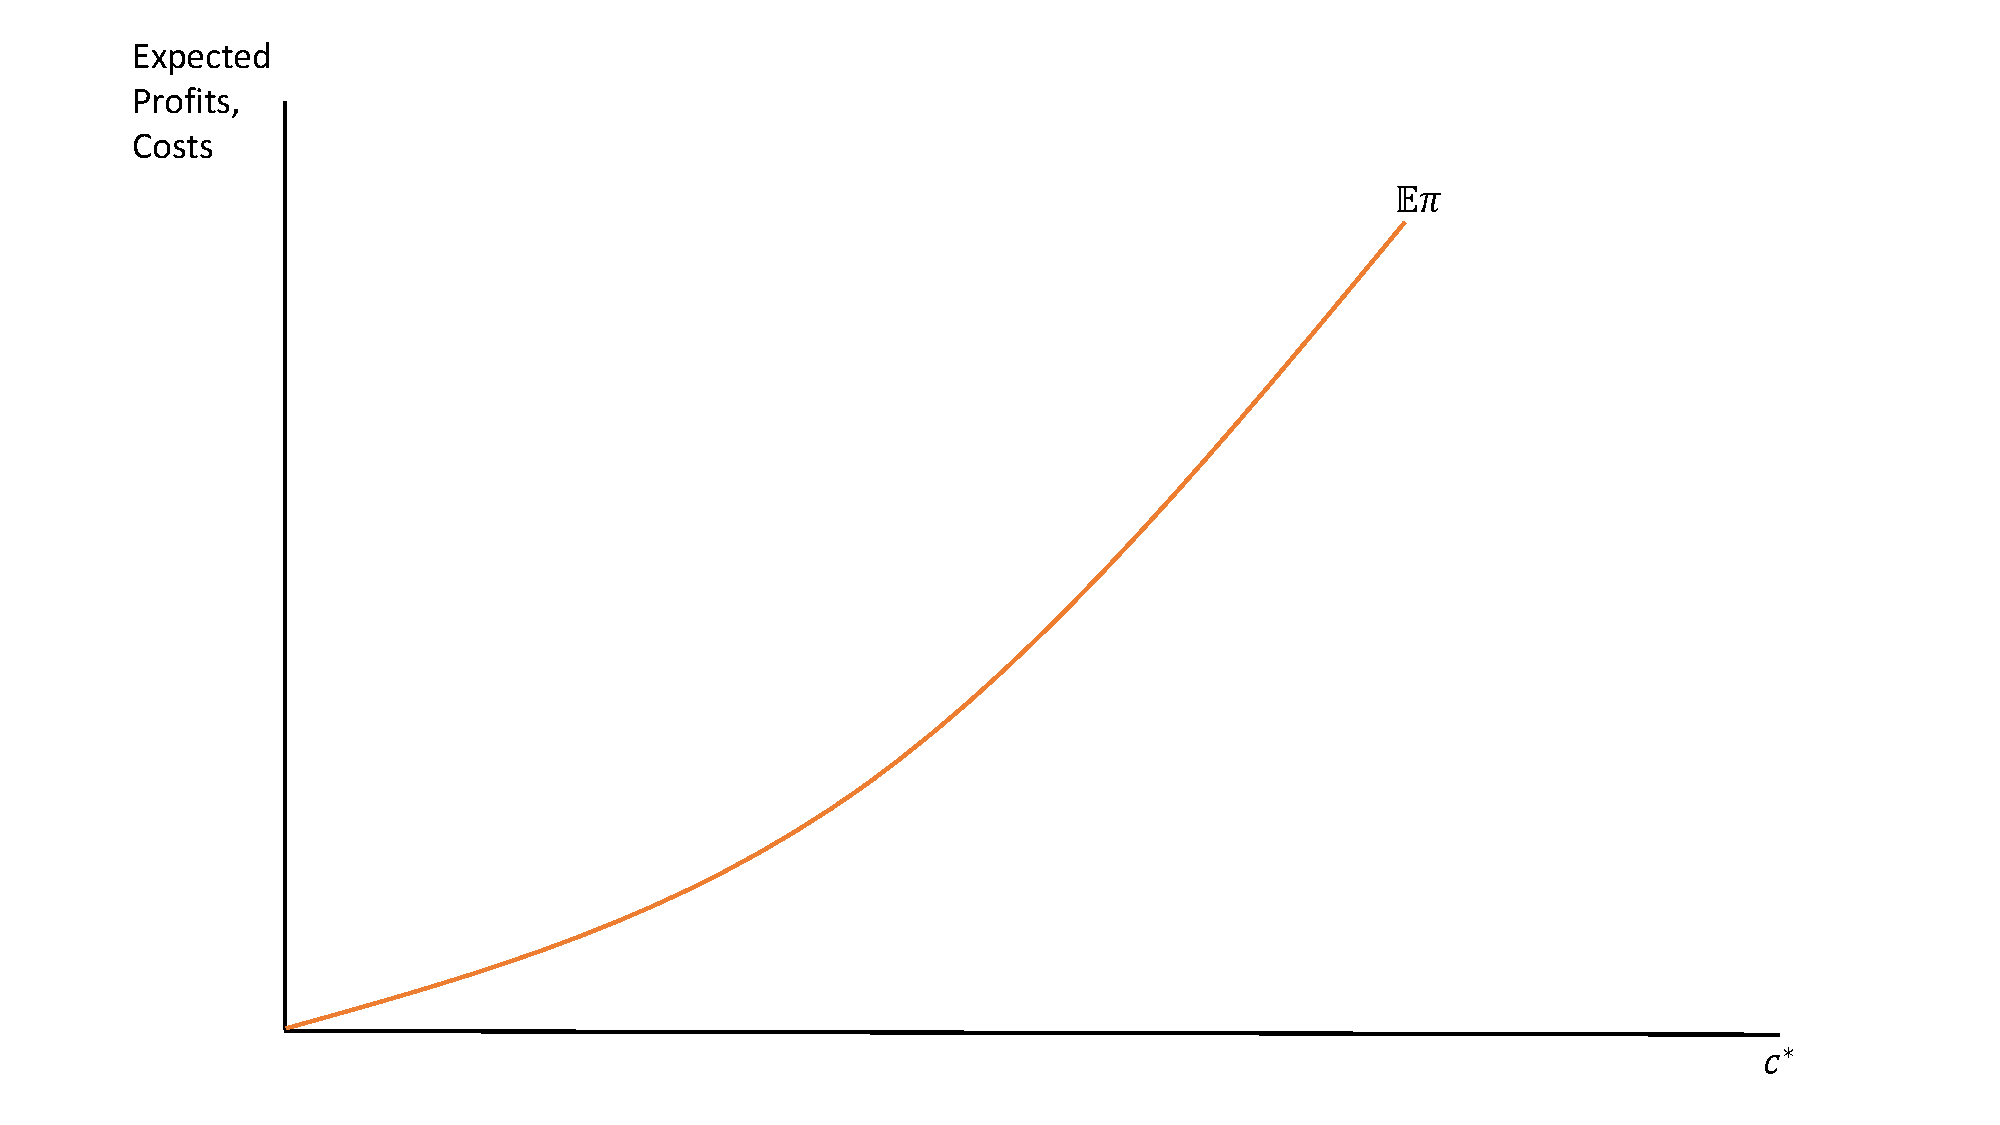
\includegraphics[scale=0.32]{SL3_3.pdf}
\end{frame}

\begin{frame}
	\frametitle{To try and obtain these profits, need to pay K}
	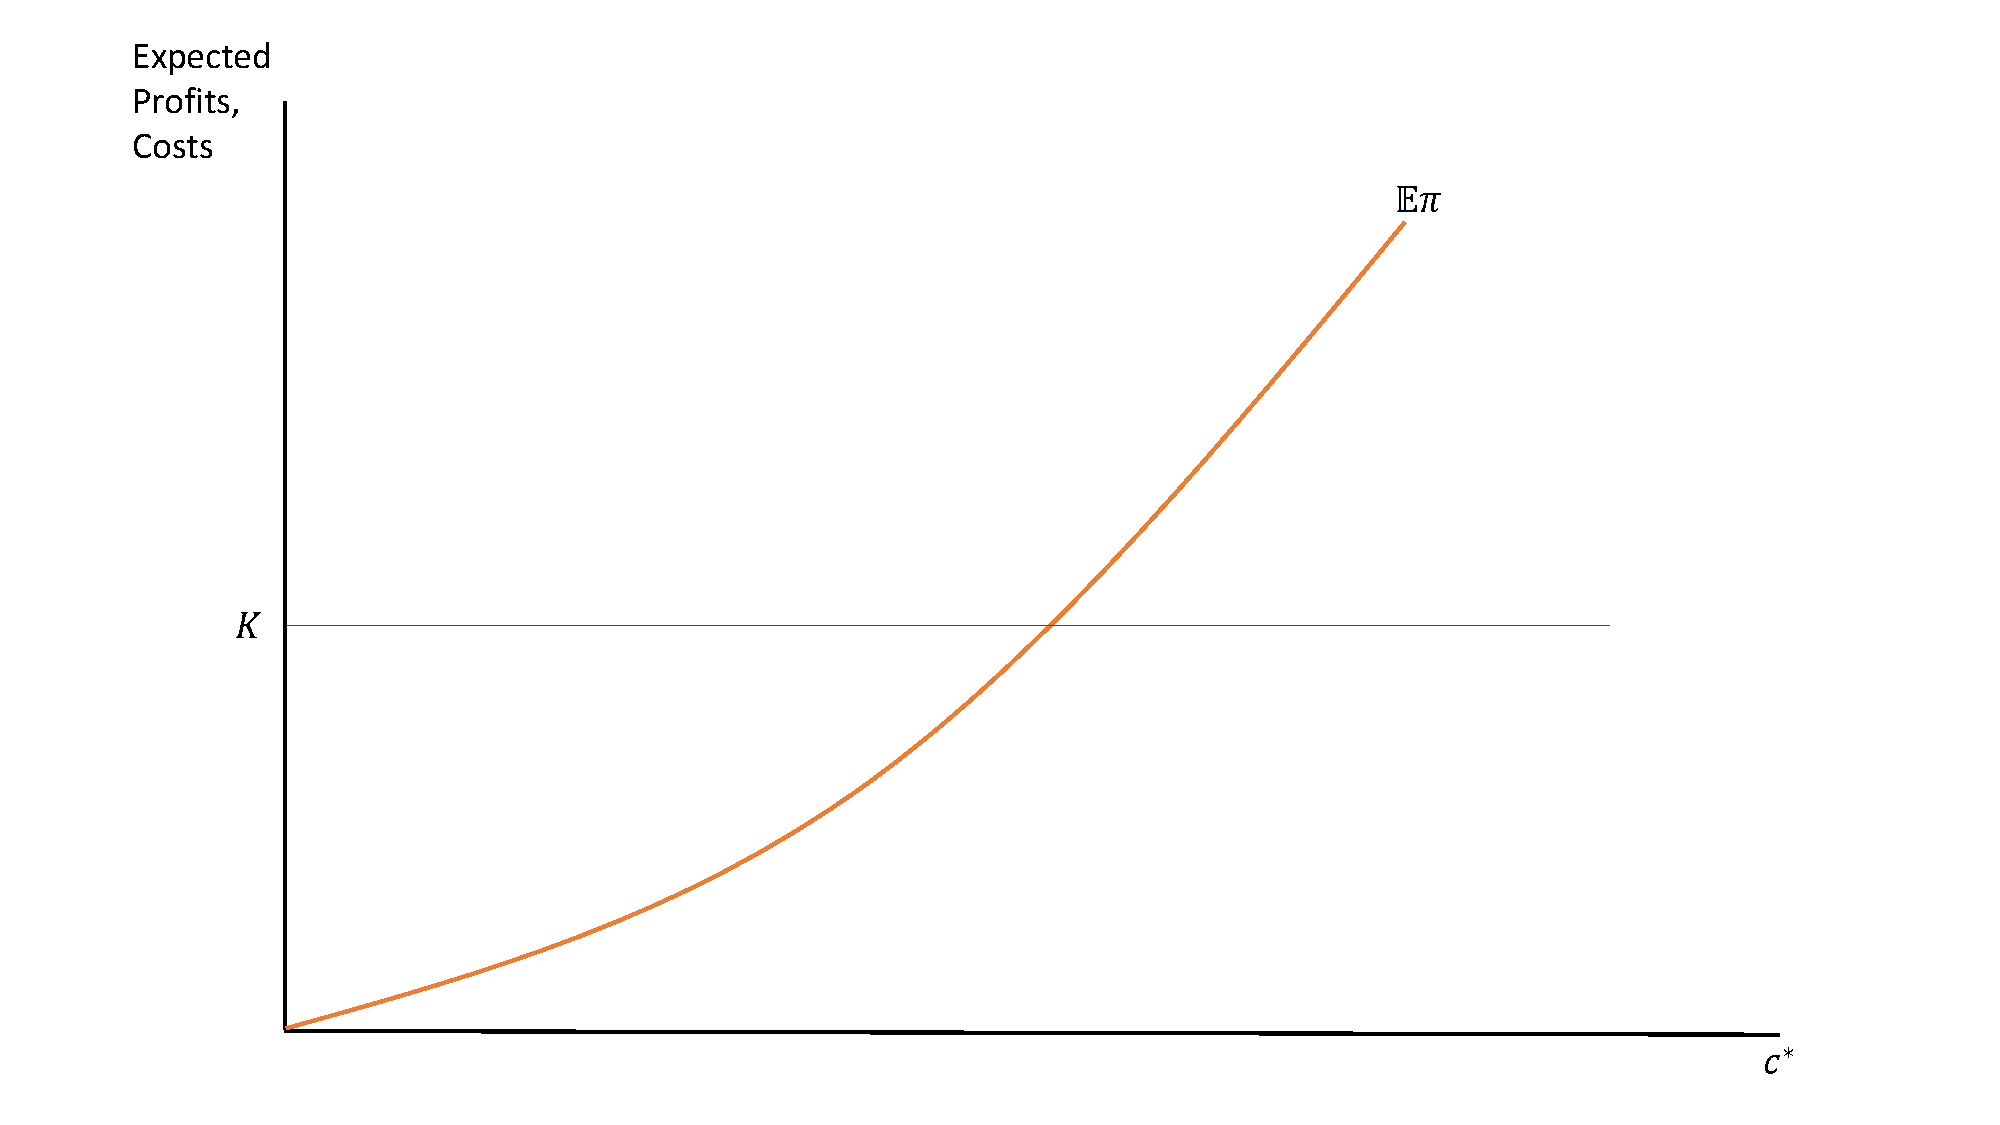
\includegraphics[scale=0.32]{SL3_4.pdf}
\end{frame}

\begin{frame}
	\frametitle{In equilibrium, expected profits = K}
	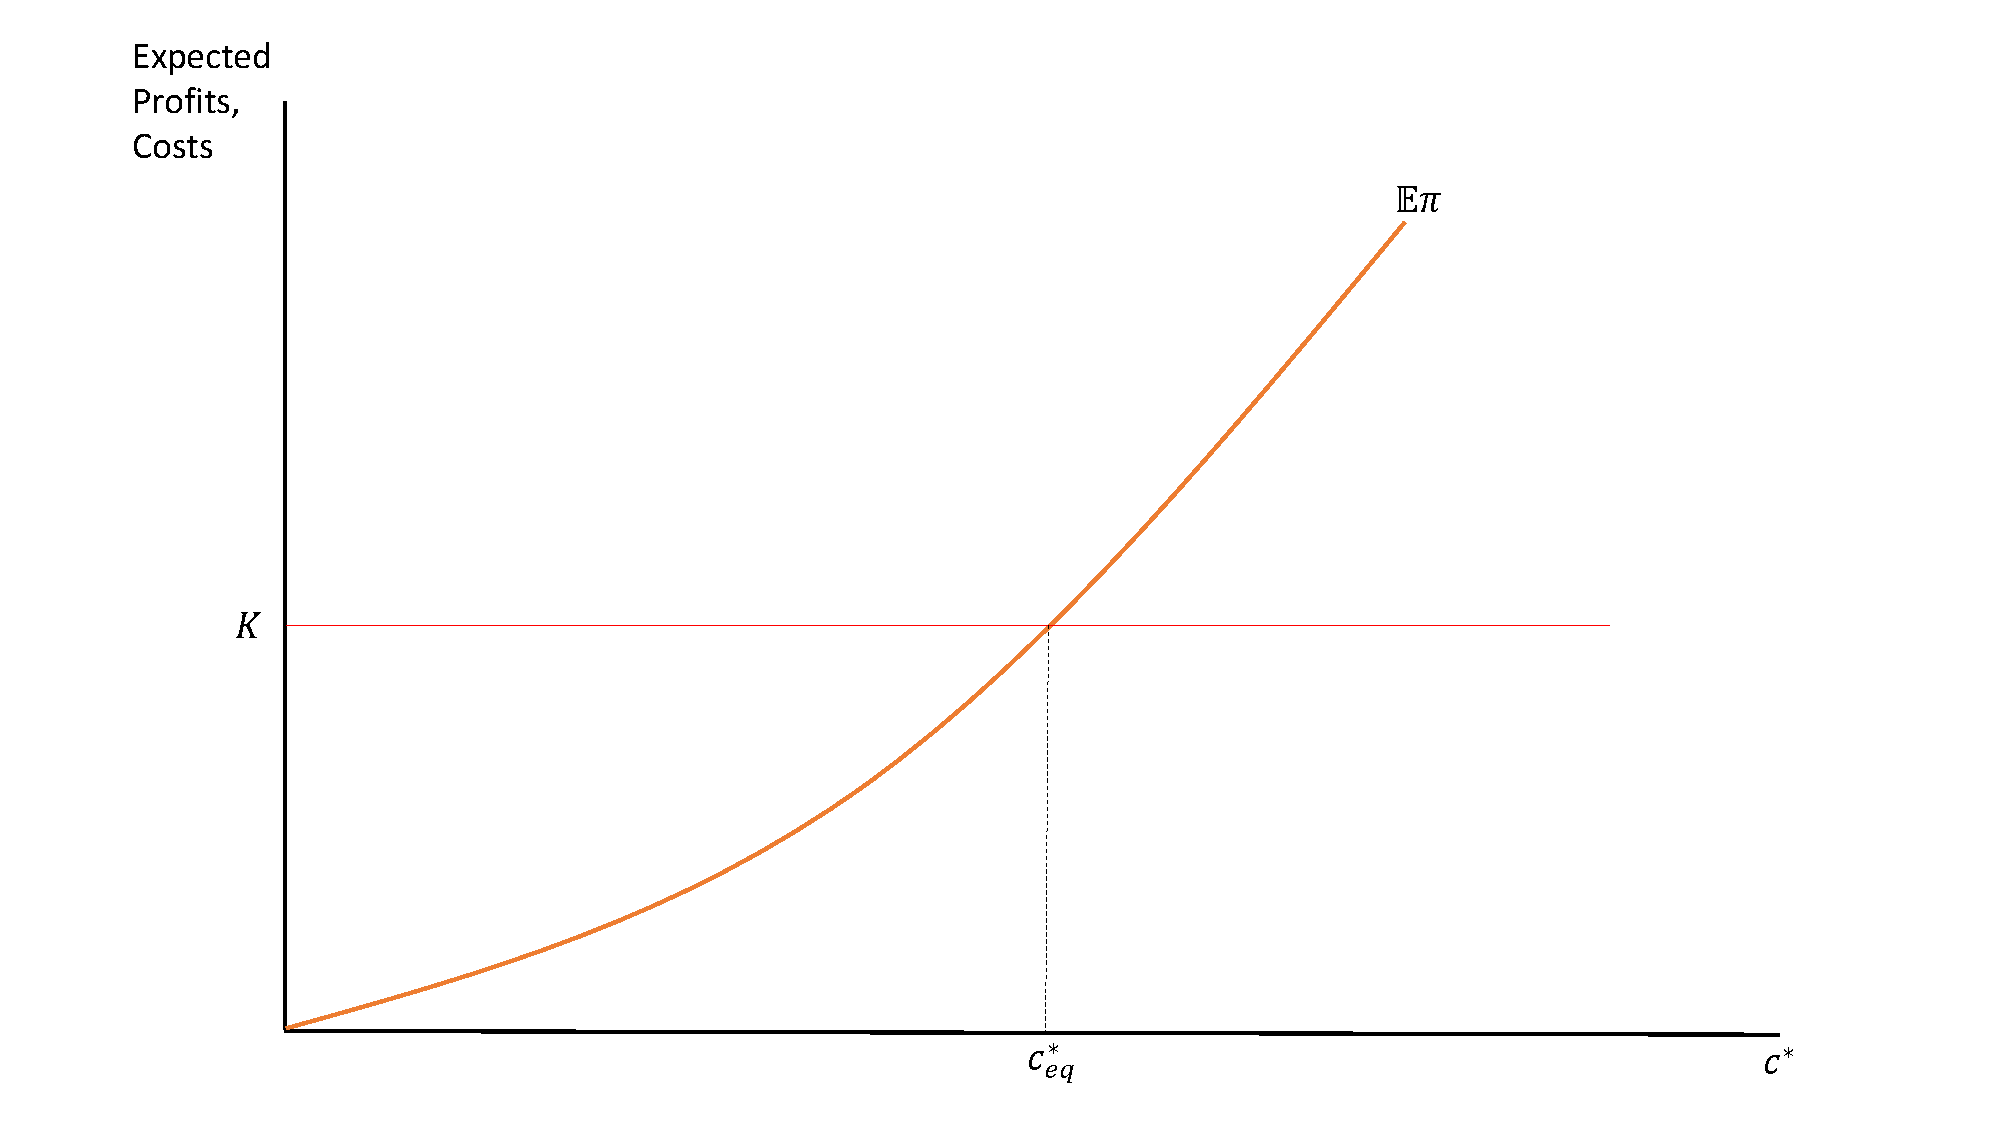
\includegraphics[scale=0.32]{SL3_5.pdf}
\end{frame}

\begin{frame}[label=cost2]
	\frametitle{Trade and Competition}
Zero expected profit condition pins down $c^*=\frac{1}{bn}+\bar{p}$, which pins down the level of competition.
	\begin{itemize}
		\item What does trade integration ($\uparrow S$) do to $c^*$?
			\begin{itemize}
				\item Increased market size rotates the expected profit curve upwards \hyperlink{Formal2}{\beamerbutton{Formal Demonstration}}
					\begin{itemize}
						\item Increased market size increases profits for all potential levels of $c^*$ 
						\item ...except $c^*=0$ (Since nobody will stay in the market in this case!)
					\end{itemize}
			\end{itemize}
		\item End result: $c^*$ has to fall.
	\end{itemize}
\end{frame}

\begin{frame}
	\frametitle{Impact of trade on cost cutoffs}
			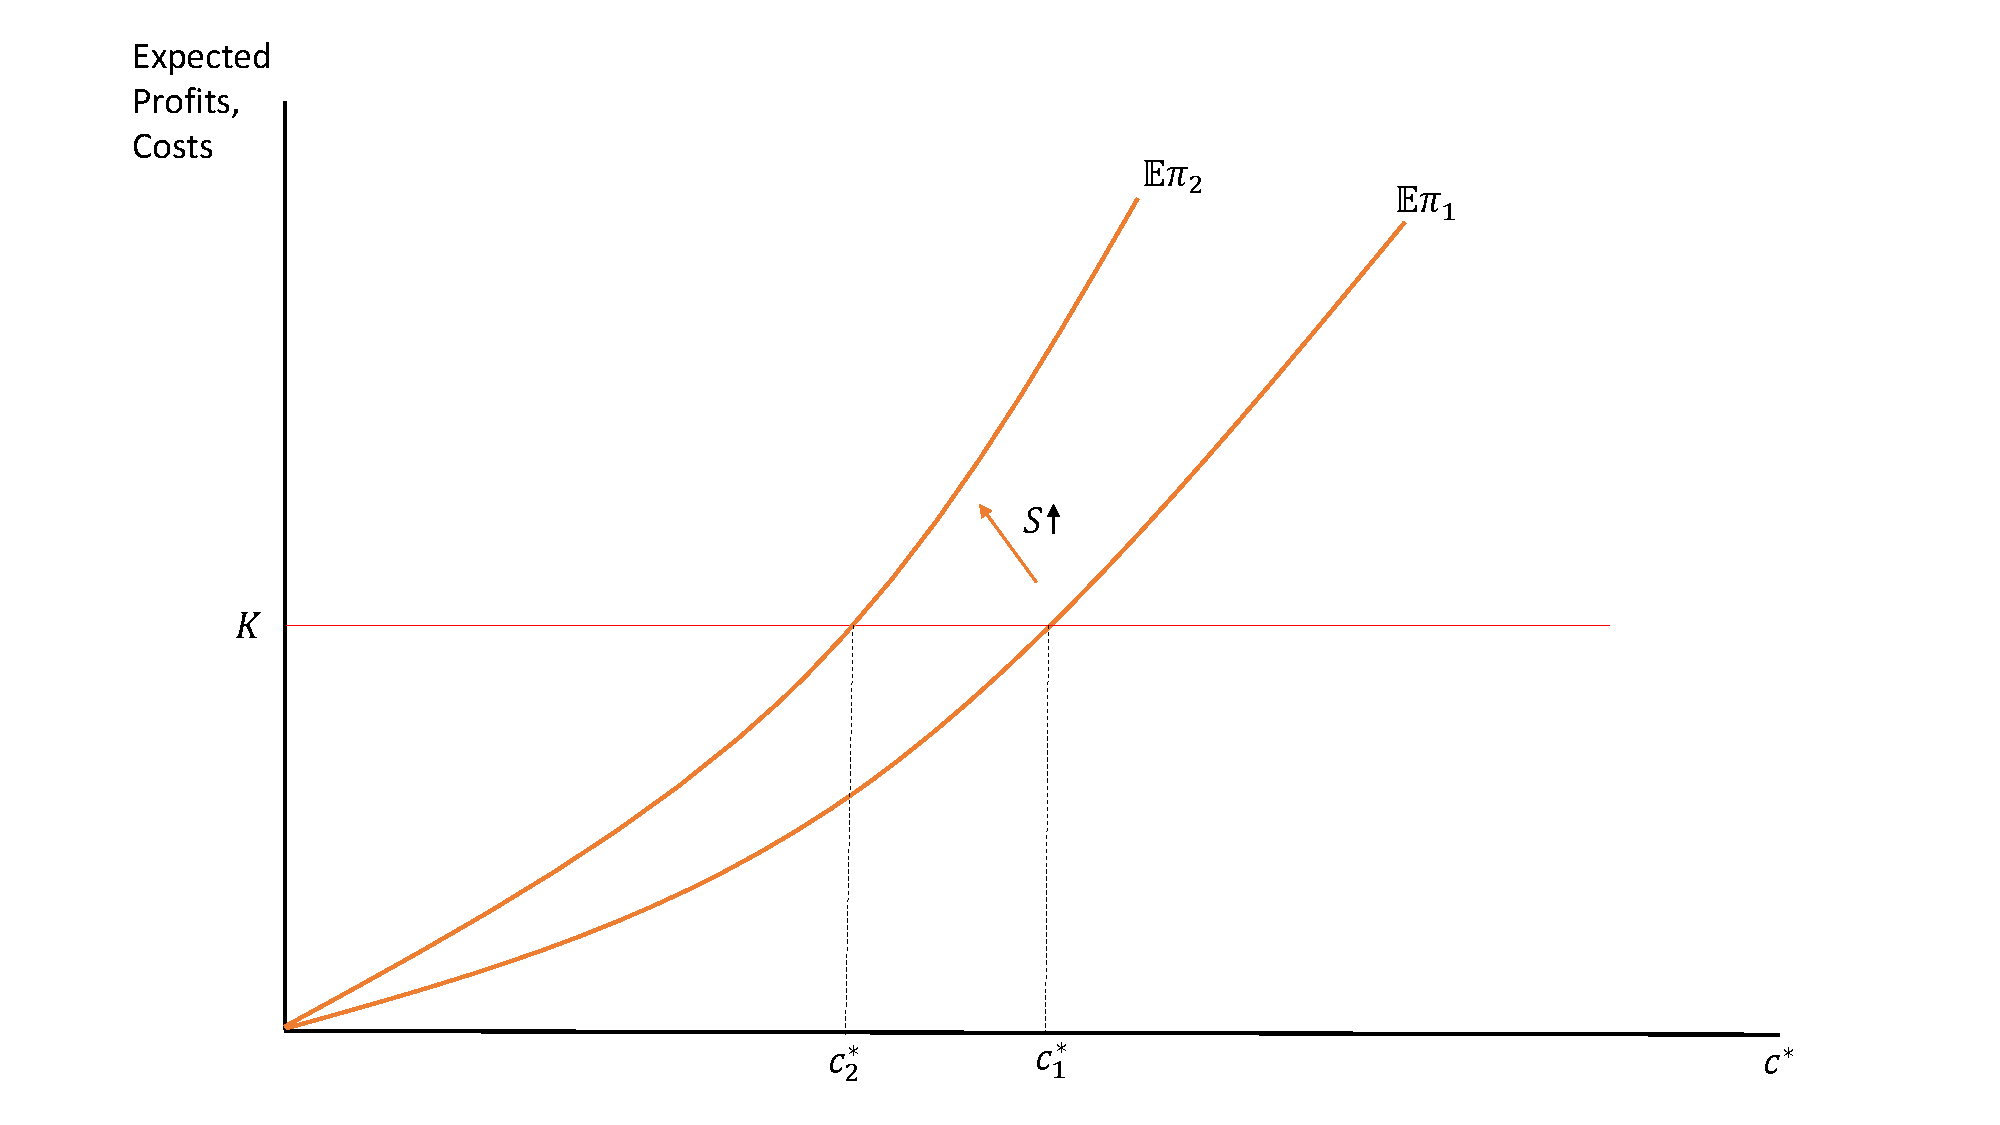
\includegraphics[scale=0.32]{SL3_6.pdf}
\end{frame}

\begin{frame}
	\frametitle{Overall impact of trade on competition and productivity}
We have shown that trade integration will decrease the marginal cost cutoff $\rightarrow$ less productive firms will definitely exit the market. 
	\begin{itemize}
		\item Moreover, since $c^*=\frac{1}{bn} +\bar{p}$, ``competition" (as measured by the inverse demand intercept) needs to increase.
			\begin{itemize}
				\item Either $n \uparrow$ or $\bar{p} \downarrow $ (or both!)
					\begin{itemize}
						\item ...Although it is somewhat difficult to pin down what will happen to each endogenous variable separately.
					\end{itemize}
			\end{itemize}
		\item Key point: Model with endogenous entry still generates the demand rotation, generating winners are losers due to trade.
			\begin{itemize}
				\item Generates some exit, just like the homogeneous firm model, but now we see that it is only the \emph{least productive firms} that exit the market.
				\item Generates \emph{allocative efficiency gains}
			\end{itemize}
	\end{itemize}

\end{frame}


\begin{frame}
	\frametitle{Summary}
Today we covered:
\begin{itemize}
	\item Monopolistic competition with homogeneous firms
		\begin{itemize}
			\item New gains from trade:
				\begin{itemize}
					\item Gains from variety $n\uparrow$
					\item Pro-competitive gains $\mu \downarrow $ and $p \downarrow$
					\item Efficiency gains: $AC \downarrow$
				\end{itemize}
		\end{itemize}
		\item Monopolistic competition with heterogeneous firms
		\begin{itemize}
			\item New gains from trade:
			\begin{itemize}
			\item Allocative productivity gains $c^* \downarrow $
			\end{itemize}
		\end{itemize}
\end{itemize}
Next Class:
	\begin{itemize}
		\item Allow for increasing returns in heterogeneous firm models.
			\begin{itemize}
				\item ``Exporter Selection"
			\end{itemize}
		\item Some empirics related to new trade theories
		\item External economies of scale
		\item Trade policy with market power (monopoly)
	\end{itemize}
	
\end{frame}

\section{Optional Appendix}

\begin{frame}[label=Formal]
	\frametitle{Expected Profits increase with $c^*$ (Optional)}
Key Condition:
\begin{equation}
\mathbb{E}\left[\pi \right] = \int_0^{c^*}\pi(c)f(c)dc=K  \nonumber 
\end{equation}	
\begin{itemize}
	\item Substitute the cost-cutoff equation into our profit equation
	\begin{equation}
	\pi(c_j)=\frac{S}{4}\left(\frac{1}{bn}+\bar{p} -c_j \right)^2 =  \frac{S}{4}\left(c^*-c_j \right)^2 \nonumber
	\end{equation}
	\item Substitute profits into zero expected profit condition.
	\begin{equation}
	\mathbb{E}\left[\pi \right] = \frac{S}{4}\int_0^{c^*}\left(c^*-c_j \right)^2 f(c)dc=K  \nonumber 
	\end{equation}
	\item LHS is clearly increasing with $c^*$

\end{itemize}
	
	\hyperlink{cost}{\beamerbutton{Back}}
\end{frame}


\begin{frame}[label=Formal2]
	\frametitle{Expected Profits increase with $c^*$ (Optional)}
	Key Condition:
	\begin{equation}
	\mathbb{E}\left[\pi \right] = \int_0^{c^*}\pi(c)f(c)dc=K  \nonumber 
	\end{equation}	
	\begin{itemize}
		\item Substitute the cost-cutoff equation into our profit equation
		\begin{equation}
		\pi(c_j)=\frac{S}{4}\left(\frac{1}{bn}+\bar{p} -c_j \right)^2 =  \frac{S}{4}\left(c^*-c_j \right)^2 \nonumber
		\end{equation}
		\item Substitute profits into zero expected profit condition.
		\begin{equation}
		\mathbb{E}\left[\pi \right] = \frac{S}{4}\int_0^{c^*}\left(c^*-c_j \right)^2 f(c)dc=K  \nonumber 
		\end{equation}
		\item LHS is clearly increasing with $c^*$
		\begin{itemize}
			\item LHS rotates upwards from the origin if $S\uparrow $
		\end{itemize}
		
	\end{itemize}
	
	\hyperlink{cost2}{\beamerbutton{Back}}
\end{frame}


\end{document}